\section{Experimental Evaluation}
\label{sec:expts}
\newcommand{\census}{\texttt{USCensus1990}\xspace}
\newcommand{\uscensus}{\texttt{USCensus1990}\xspace}
\newcommand{\tower}{\texttt{Tower}\xspace}
\newcommand{\covtype}{\texttt{Covtype}\xspace}
\newcommand{\power}{\texttt{Power}\xspace}
\newcommand{\intrusion}{\texttt{Intrusion}\xspace}
\newcommand{\drift}{\texttt{Drift}\xspace}


This section describes an empirical study of the proposed algorithms, in
comparison to the state-of-the-art clustering algorithms.  Our goals are
twofold: to understand the clustering accuracy and the running time of
different algorithms in the context of continuous queries, and to investigate
how they behave under different settings of algorithm parameters.

%---------------------------------------------
\subsection{Datasets}
%---------------------------------------------
Our experiments use a number of real-world or semi-synthetic datasets, based on
data from the UCI Machine Learning Repositories~\cite{Lichman13}.  These are
commonly used datasets in benchmarking clustering
algorithms. Table~\ref{table:dataset} provides an overview of the datasets used.

The \textit{\covtype} dataset models the forest cover type prediction problem
from cartographic variables. The dataset contains $581,012$ instances and $54$
integer attributes. The \textit{\power} dataset measures electric power
consumption in one household with a one-minute sampling rate over a period of
almost four years. We remove entries with missing values, resulting in a dataset
with $2,049,280$ instances and $7$ floating-point attributes. The
\textit{\intrusion} dataset is a $10\%$-subset of the \emph{KDD Cup 1999}
data. The task was to build a predictive model capable of distinguishing between
normal network connections and intrusions. After ignoring symbolic attributes,
we have a dataset with $494,021$ instances and $34$ floating-point
attributes. To erase any potential special ordering within data, we randomly
shuffle each dataset before using it as a data stream.

However, each of the above datasets, as well as most datasets used in previous
works on streaming clustering, is not originally a streaming dataset; the
entries are only read in some order and consumed as a stream.  
To better model the evolving nature of data streams and the drifting of center locations, 
we generate a semi-synthetic dataset, called \drift, which we derive from the \census
dataset~\cite{Lichman13} as follows: The method is inspired by
Barddal~\cite{BGE+16}.  The first step is to cluster the \census dataset to
compute $20$ cluster centers and for each cluster, the standard deviation of the
distances to the cluster center.  Following that, the synthetic dataset is
generated using the Radial Basis Function (RBF) data generator from the MOA
stream mining framework~\cite{BHK+10}. The RBF generator moves the drifting
centers with a user-given direction and speed. For each time step, the RBF
generator creates $100$ random points around each center using a Gaussian
distribution with the cluster standard deviation. In total, the synthetic
dataset contains $200,000$ and $68$ floating-point attributes.

%------------
\begin{table}
{ 
\centering
\setlength{\tabcolsep}{3pt}
\begin{tabular}
{l  c  c  l}
\toprule
Dataset & Number of Points & Dimension & Description\\ 
\midrule
\covtype & $581,012$ & $54$ & forest cover type\\
\power & $2,049,280$ & $7$ & household  power consumption \\
\intrusion & $494,021$ & $34$ & KDD Cup 1999\\
\drift & $200,000$ & $68$ & derived from US Census 1990\\
\bottomrule
\end{tabular}\par
\smallskip
\caption{An overview of the datasets used in the experiments.}
\label{table:dataset}
}
\end{table}
%----------


%-------------------------------
\subsection{Experimental Setup and Implementation Details}
%-------------------------------
% Describe the machine used, compiler, etc.
We implemented all the clustering algorithms in Java, and ran experiments on a
desktop with Intel Core i5-4460 $3.2$GHz processor and $8$GB main memory.

\noindent\textbf{Algorithms:} Our baseline algorithms are two prominent streaming
clustering algorithms. (1)~the \seqkm algorithm due to
MacQueen~\cite{MacQueen67}, which is frequently implemented in clustering
packages today. For \seqkm clustering, we use the implementation in Apache Spark
MLLib~\cite{MBY+15}, though ours is modified to run sequentially. Furthermore,
the initial centers are set by the first $k$ points in the stream instead of
setting by random Gaussians, to ensure no clusters are empty. (2)~We also
implemented \skmpp~\cite{AMR+12}, a current state-of-the-art algorithm that has
good practical performance.  \skmpp can be viewed as a special case of \ct where
the merge degree $r$ is $2$. The bucket size is $20 \cdot k$, where $k$ is the number
of centers. \footnote{A larger bucket size such as $200k$ can yield slightly 
better clustering quality. But this led to a high runtime for \skmpp, 
especially when queries are frequent, so we use a smaller bucket size.}

For \cc, we set the merge degree to $2$, in line with \skmpp. For \rcc, we use a
maximum nesting depth of $3$, so the merge degrees for different structures are
$N^{\frac{1}{2}}, N^{\frac{1}{4}}$ and $N^{\frac{1}{8}}$, respectively. For
\hybrid, the threshold $\alpha$ is set to $1.2$ by default. 

\remove{
To compute the $\estcost$ after
each fallback to \cc, we need to know the value of the clusters' standard
deviation $D$. This value is estimated using the coreset which is representative
of the whole data received.
}

We use the batch \kmpp algorithm as the baseline for clustering accuracy. This
is expected to outperform any streaming algorithm, as with the scope of all the points.  
The \kmpp algorithm, similar to~\cite{AMR+12,AJM09}, is used to derive coresets.  
We also use \kmpp as the final step to construct $k$ centers from the coreset, 
and take the best clustering out of five independent runs of \kmpp; 
each run of \kmpp is followed by up to $20$ iterations of Lloyd's algorithm to 
further improve clustering quality.
Finally, for each statistic, we report the median value from five independent runs 
of each algorithm to improve robustness. The queries on cluster centers present with interval of $q$ points. 
Hence, from the beginning of the stream, there is one query per $q$ input points received. 
By default, the number of clusters is set to $30$, the query interval is set to $100$ points.
In order to test the algorithm performance in a more practical way of presenting queries, 
we also generate a stream of queries in the poisson process. 
Let $\lambda$ be the arrival rate of poisson process. 
Based on the definition of poisson process, the inter arrival time between query events 
should be an exponential distribution variable with mean of $\frac{1}{\lambda}$. 
We set the inter arrival of queries in range of $\{50, 100, 200, 400, 800, 1600, 3200 \}$ points.

\noindent\textbf{Metrics:} 
We use three metrics: clustering accuracy, runtime and memory cost. 
The clustering accuracy is measured using the \km cost, also known as the
within cluster sum of squares (SSQ).  We measure the average runtime of the
algorithm per point, as well as the total runtime over the entire stream. 
The runtime contains two parts, (1)~update time, the time required to update internal
data structures upon receiving new point, and (2)~query time, the time required
to answer clustering queries.  Finally, we consider the memory consumption
through measuring the number of points stored by the internal data structure, 
including both the coreset tree and coreset cache. From the number of points, 
we estimate the number of bytes used, assuming that each dimension of 
a data point consumes $8$ bytes (size of a double-precision floating-point number).

%---------------------------
%\subsection{Results}
%---------------------------
%Plots showing performance of different methods.

% metrics vs. stream
%%----------------
\begin{figure*}
  \centering
  \subfloat[\covtype]{
  \centering 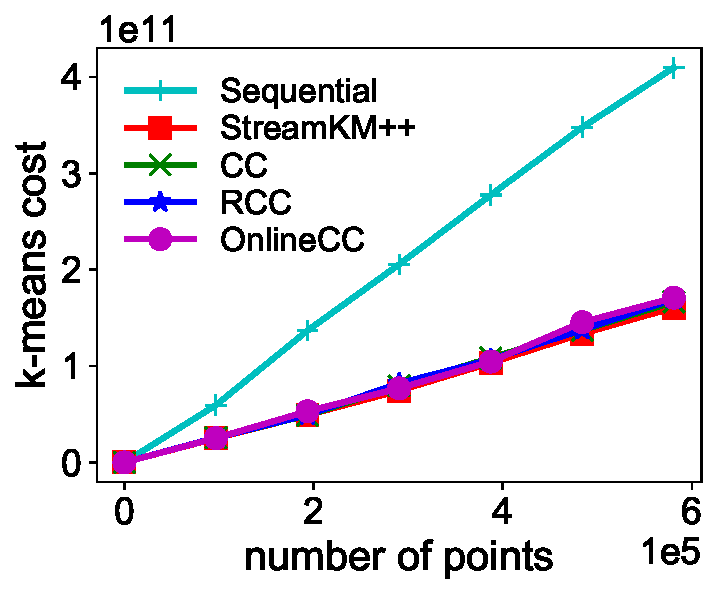
\includegraphics[width=0.23\textwidth]{expfigs/accuracy_num/covtype_cost_vs_num.pdf}
  }
  \subfloat[\power]{
  \centering 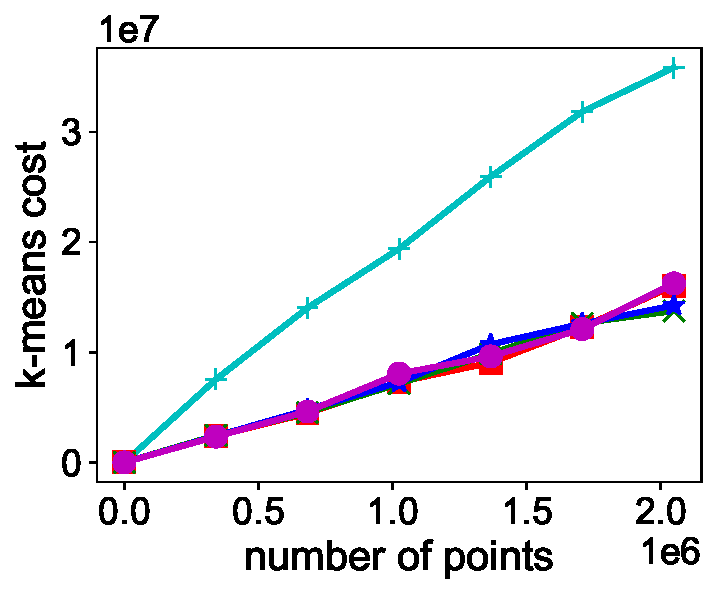
\includegraphics[width=0.23\textwidth]{expfigs/accuracy_num/power_cost_vs_num.pdf}
  }
  \subfloat[\intrusion  (\seqkm not shown)]{
  \centering 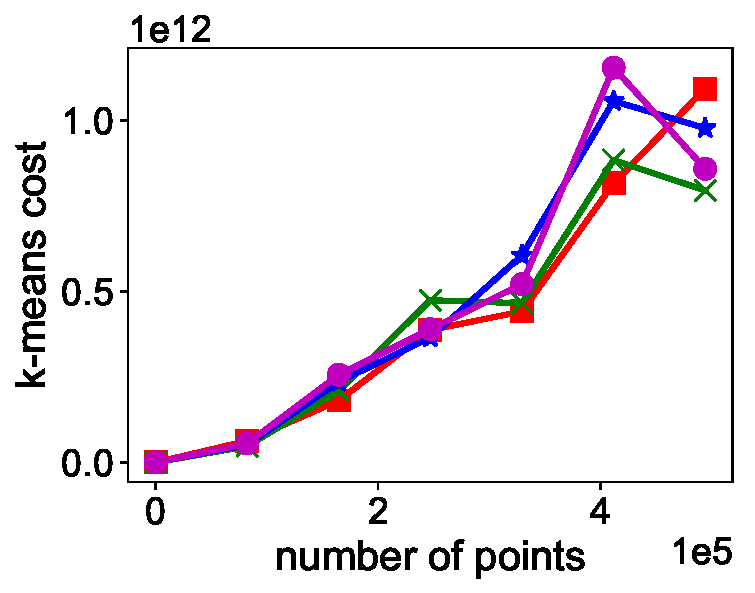
\includegraphics[width=0.23\textwidth]{expfigs/accuracy_num/intrusion_cost_vs_num.pdf}
  }
  \subfloat[\drift]{
  \centering 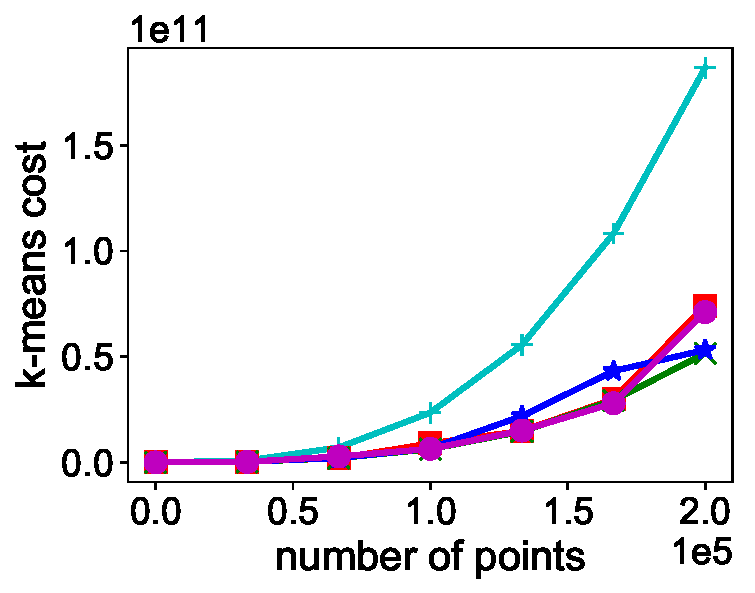
\includegraphics[width=0.23\textwidth]{expfigs/accuracy_num/synthetic_cost_vs_num.pdf}
  }
\caption{\km cost vs. number of points. The number of clusters $k$ is $30$.}
\label{fig:cost-versus-stream}
\end{figure*}
%----------------

%----------------
\begin{figure*}
  \centering
  \subfloat[\covtype]{
  \centering 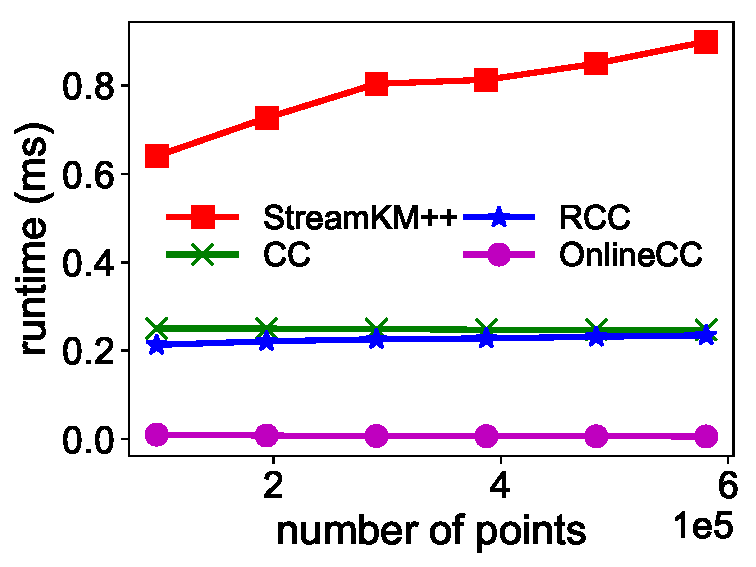
\includegraphics[width=0.23\textwidth]{expfigs/totaltime_num/covtype_total_vs_num.pdf}
  }
  \subfloat[\power]{
  \centering 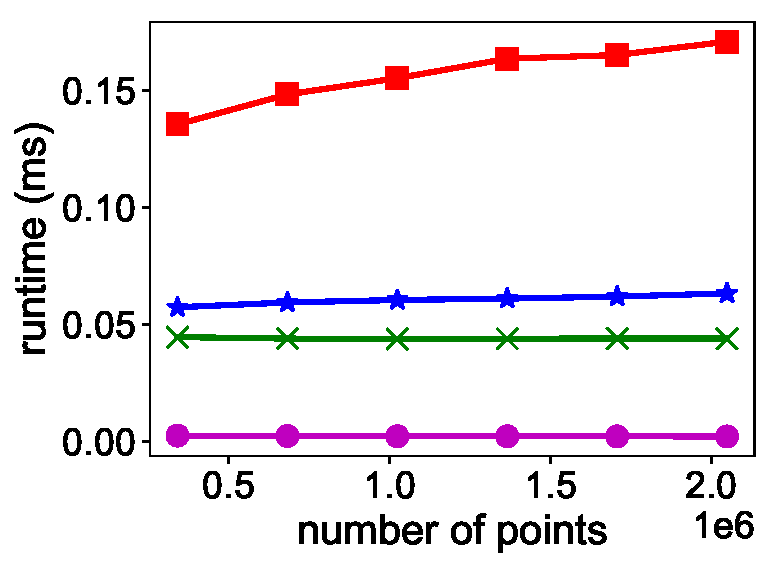
\includegraphics[width=0.23\textwidth]{expfigs/totaltime_num/power_total_vs_num.pdf}
  }
  \subfloat[\intrusion]{
  \centering 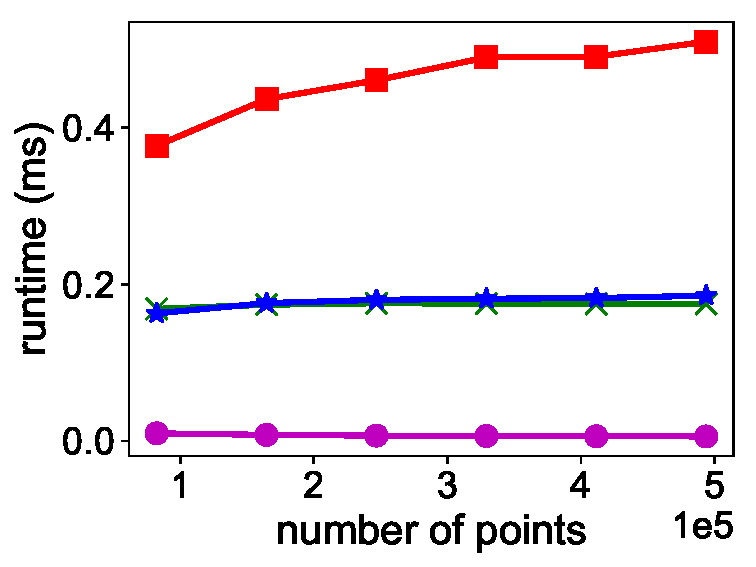
\includegraphics[width=0.23\textwidth]{expfigs/totaltime_num/intrusion_total_vs_num.pdf}
  }
  \subfloat[\drift]{
  \centering 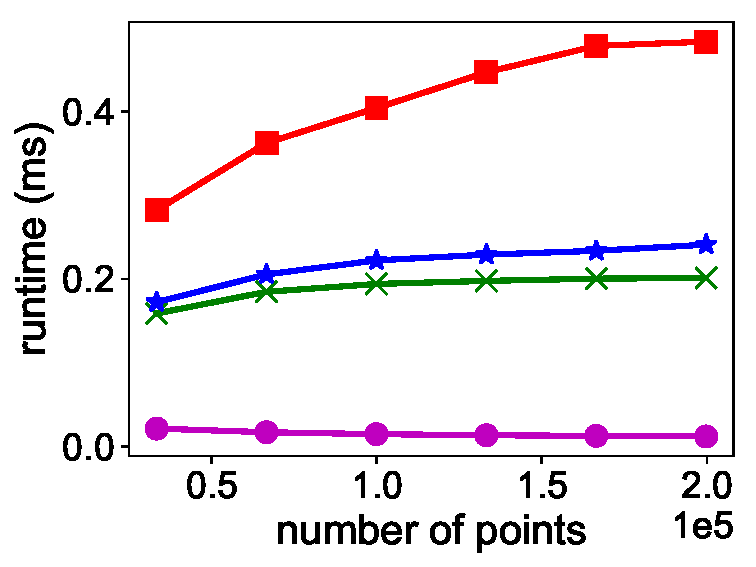
\includegraphics[width=0.23\textwidth]{expfigs/totaltime_num/synthetic_total_vs_num.pdf}
  }
  \caption{Average runtime per point (milliseconds) vs. number of points. The number of clusters $k$ is $30$.}
\label{fig:time-versus-stream}
\end{figure*}
%----------------

% metrics vs. k
%----------------
\begin{figure*}
  \centering
  \subfloat[\covtype]{
  		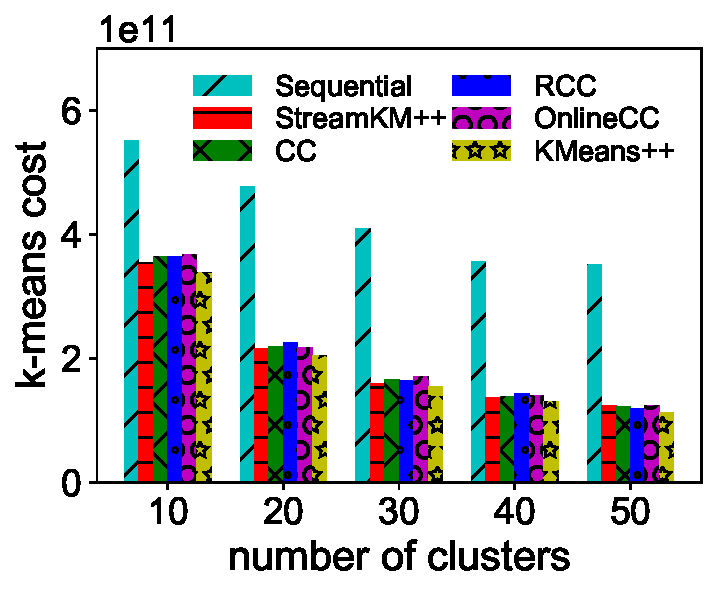
\includegraphics[width=0.24\textwidth]{expfigs/accuracy_k/covtype_cost_vs_k.pdf}
  }
  \subfloat[\power]{
  		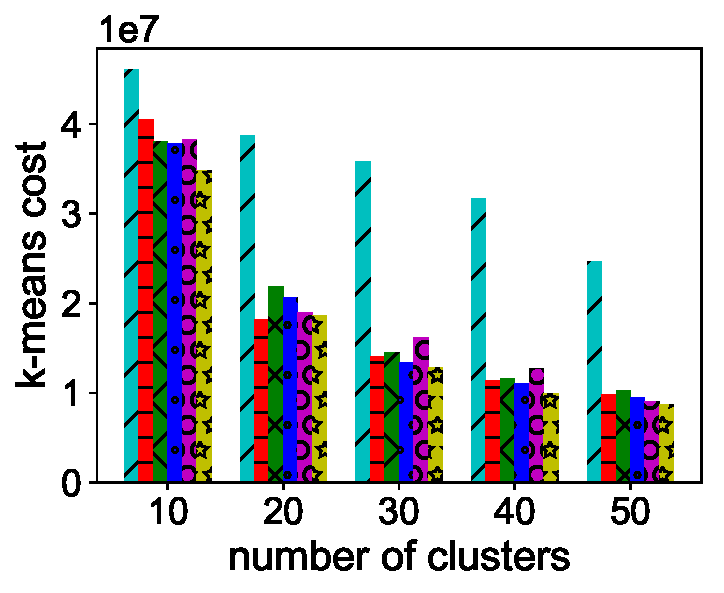
\includegraphics[width=0.24\textwidth]{expfigs/accuracy_k/power_cost_vs_k.pdf}
  }
  \subfloat[\intrusion (\km cost of \seqkm is not shown)]{
		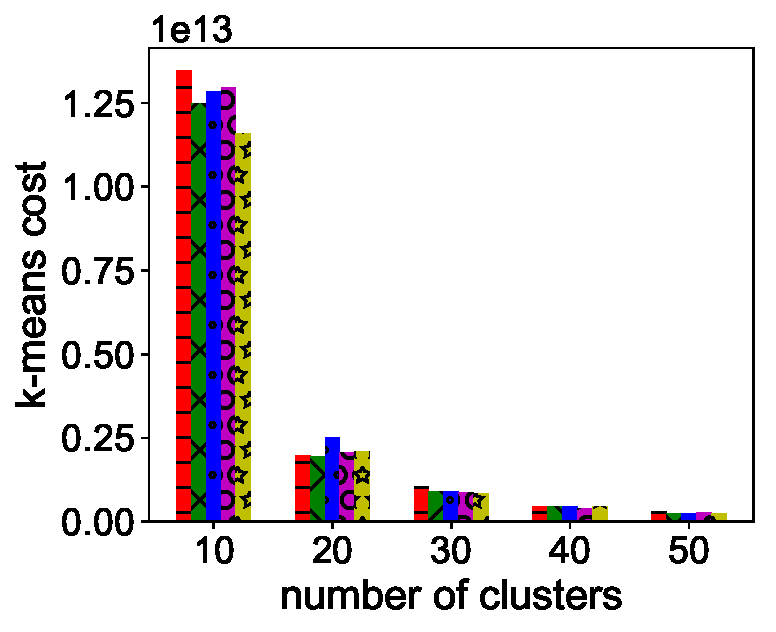
\includegraphics[width=0.24\textwidth]{expfigs/accuracy_k/intrusion_cost_vs_k.pdf}
  }
  \subfloat[\drift]{
  		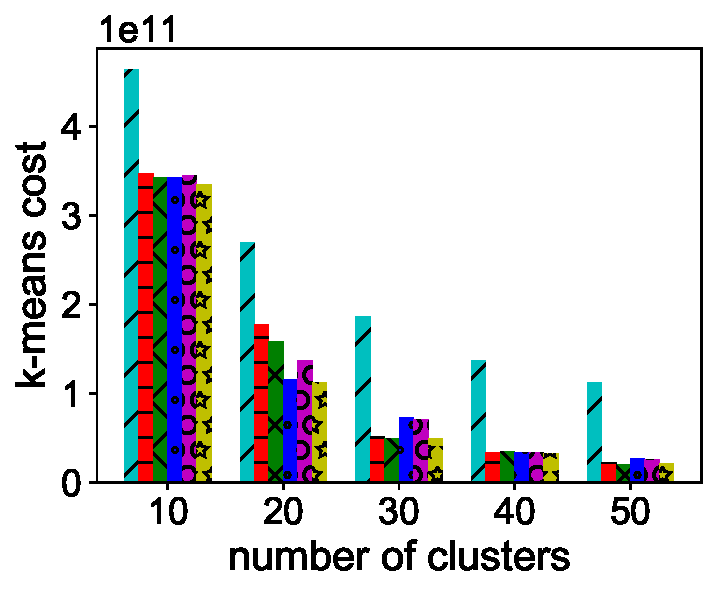
\includegraphics[width=0.24\textwidth]{expfigs/accuracy_k/synthetic_cost_vs_k.pdf}
  }
  \caption{\km cost vs. number of clusters $k$. The cost is computed at the end of observing all the points.  
\km cost of \seqkm on \intrusion dataset is not shown in Figure (c), since it was orders of magnitude larger ($10^4$) than the other algorithms.}
\label{fig:cost-versus-k}
\end{figure*}
%----------------


%----------------
\begin{figure*}
  \centering
  \subfloat[\covtype]{
  \centering 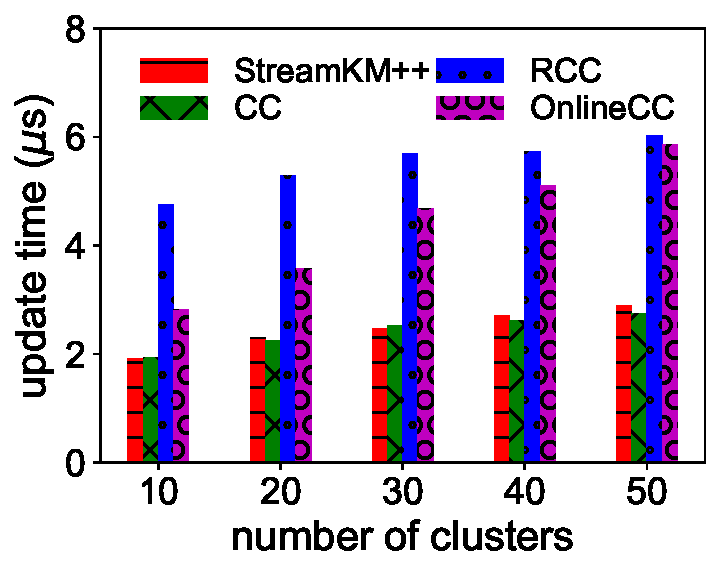
\includegraphics[width=0.23\textwidth]{expfigs/updatetime_k/covtype_update_vs_k.pdf}
  }
  \subfloat[\power]{
  \centering 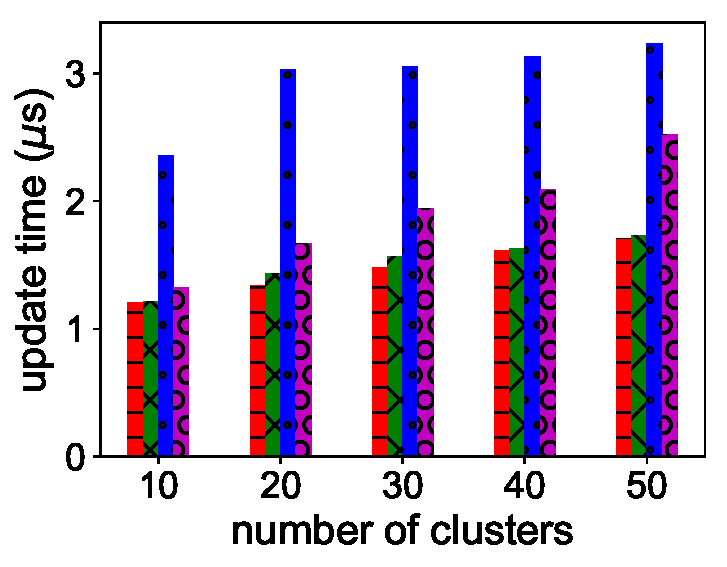
\includegraphics[width=0.23\textwidth]{expfigs/updatetime_k/power_update_vs_k.pdf}
  }
  \subfloat[\intrusion]{
  \centering 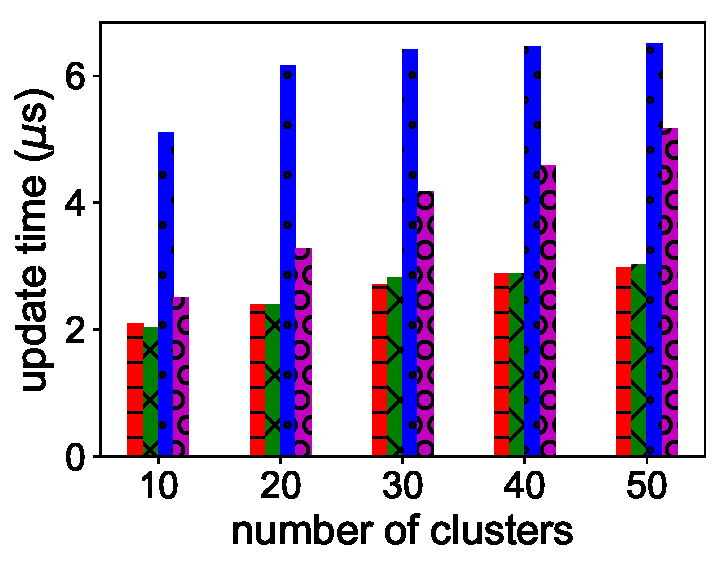
\includegraphics[width=0.23\textwidth]{expfigs/updatetime_k/intrusion_update_vs_k.pdf}
  }
  \subfloat[\drift]{
  \centering 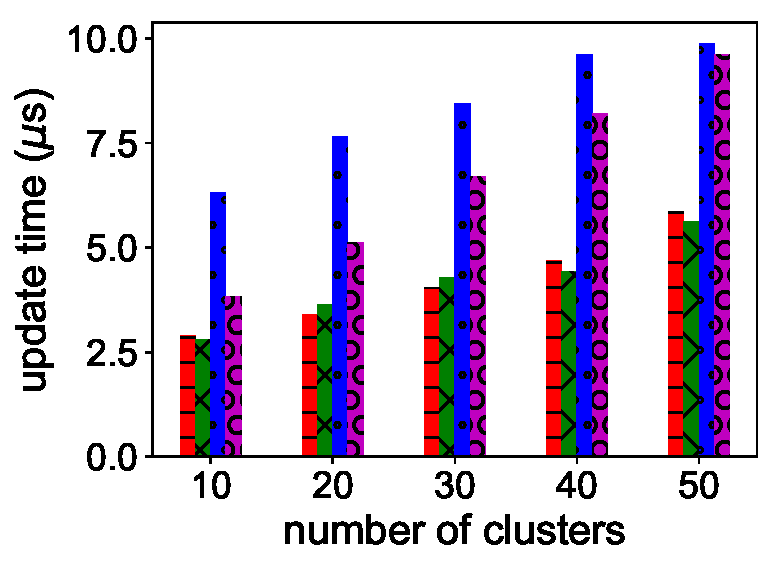
\includegraphics[width=0.23\textwidth]{expfigs/updatetime_k/synthetic_update_vs_k.pdf}
  }
  \caption{Average update time per point (microseconds)  vs. number of clusters $k$. The query interval $q$ is $100$ points.}
  \label{fig:update-versus-k}
\end{figure*}
%----------------


%----------------
\begin{figure*}
  \centering
  \subfloat[\covtype]{
  \centering 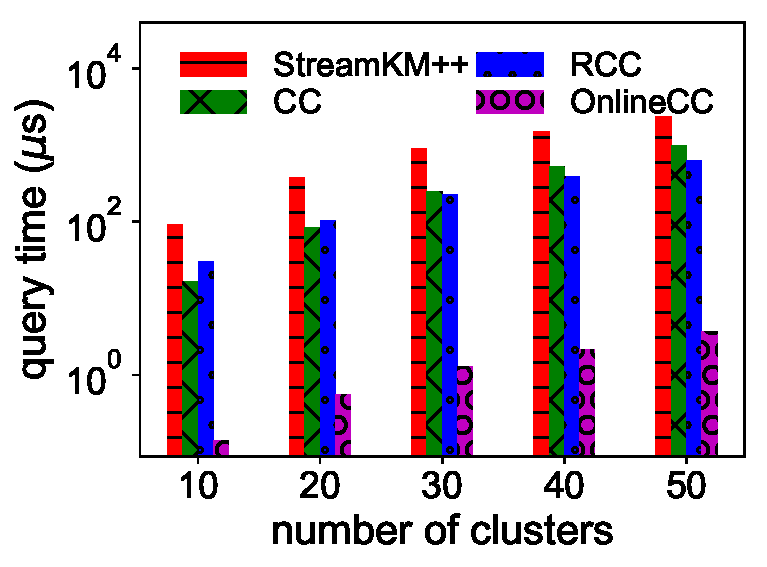
\includegraphics[width=0.23\textwidth]{expfigs/querytime_k/covtype_query_vs_k.pdf}
  }
  \subfloat[\power]{
  \centering 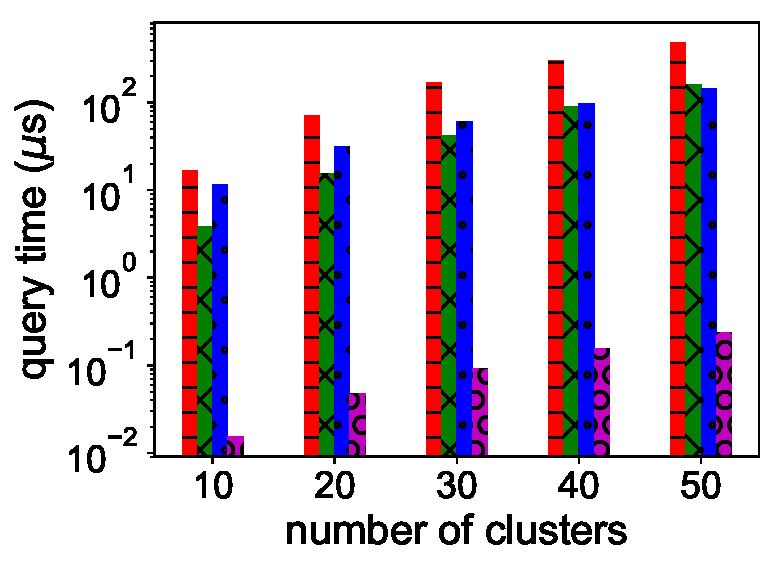
\includegraphics[width=0.23\textwidth]{expfigs/querytime_k/power_query_vs_k.pdf}
  }
  \subfloat[\intrusion]{
  \centering 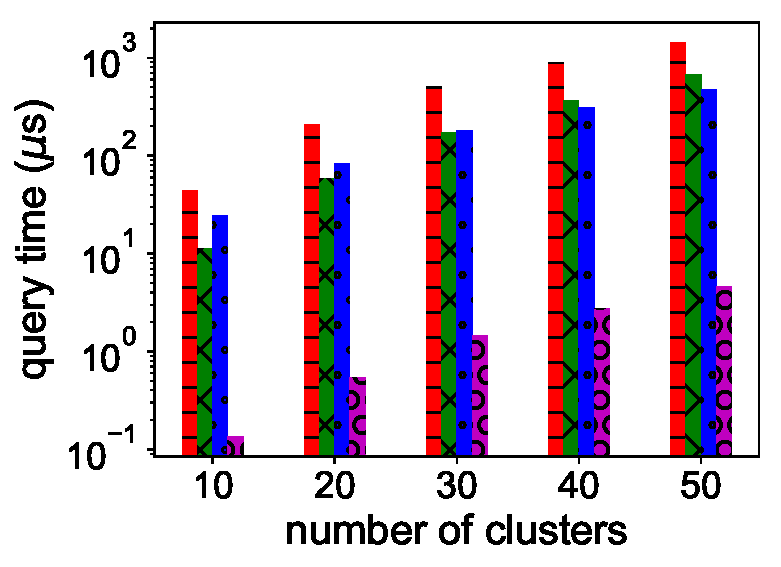
\includegraphics[width=0.23\textwidth]{expfigs/querytime_k/intrusion_query_vs_k.pdf}
  }
  \subfloat[\drift]{
  \centering 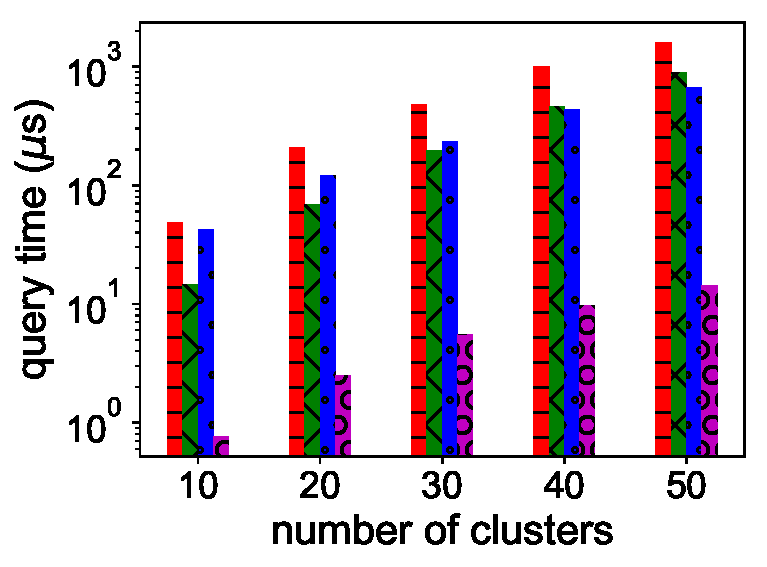
\includegraphics[width=0.23\textwidth]{expfigs/querytime_k/synthetic_query_vs_k.pdf}
  }
  \caption{Average query time per point (microseconds) vs. number of clusters $k$. The query interval $q$ is $100$ points.}
\label{fig:query-versus-k}
\end{figure*}
%----------------


%----------------
\begin{figure*}
  \centering
  \subfloat[\covtype]{
  \centering 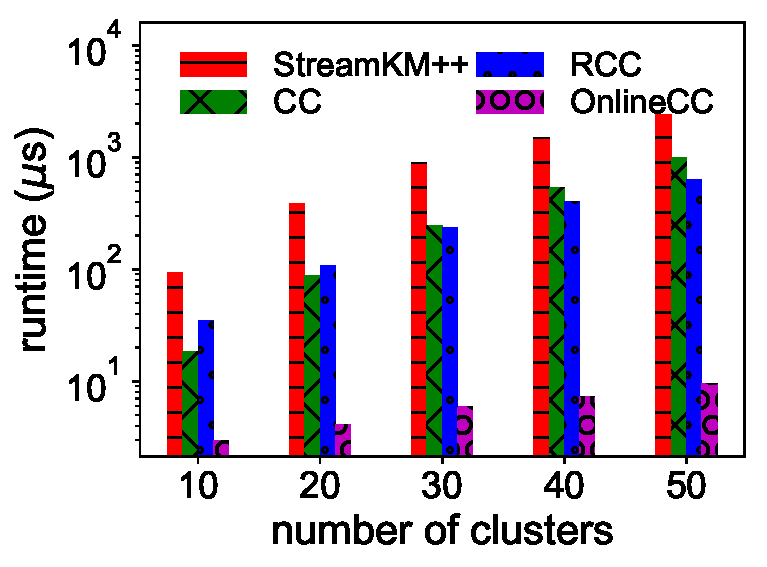
\includegraphics[width=0.23\textwidth]{expfigs/totaltime_k/covtype_total_vs_k.pdf}
  }
  \subfloat[\power]{
  \centering 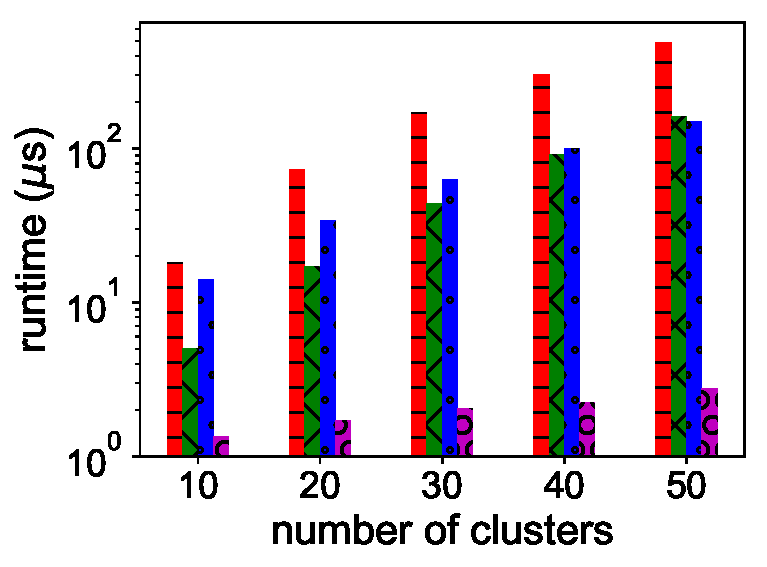
\includegraphics[width=0.23\textwidth]{expfigs/totaltime_k/power_total_vs_k.pdf}
  }
  \subfloat[\intrusion]{
  \centering 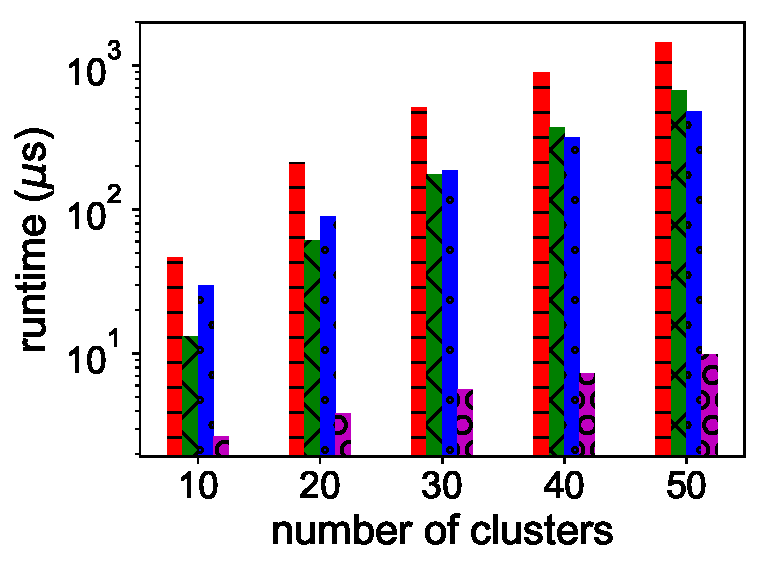
\includegraphics[width=0.23\textwidth]{expfigs/totaltime_k/intrusion_total_vs_k.pdf}
  }
  \subfloat[\drift]{
  \centering 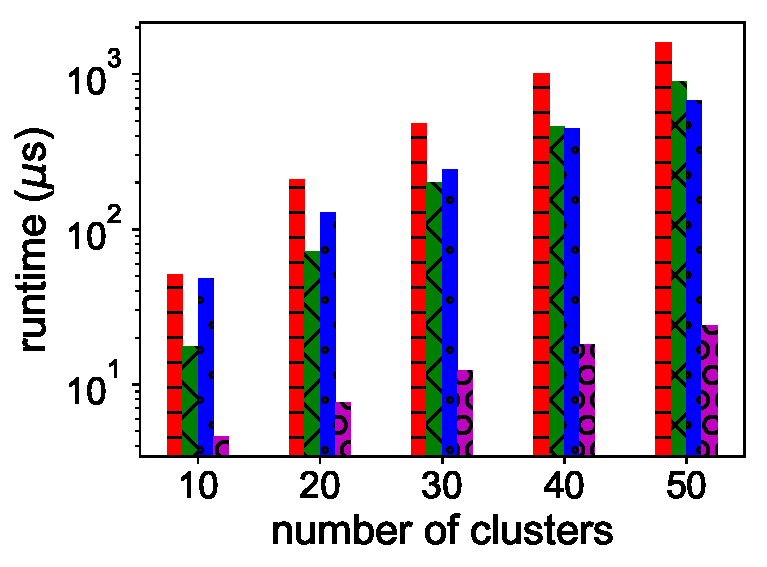
\includegraphics[width=0.23\textwidth]{expfigs/totaltime_k/synthetic_total_vs_k.pdf}
  }
  \caption{Average runtime per point (microseconds) vs. number of clusters $k$. The runtime is sum of average update time (per point) and the average query time (per point). The query interval $q$ is $100$ points.}
  \label{fig:total-versus-k}
\end{figure*}
%----------------

% metrics vs. q (query interval)
%----------------
\begin{figure*}
  \centering
  \subfloat[\covtype]{
  \centering 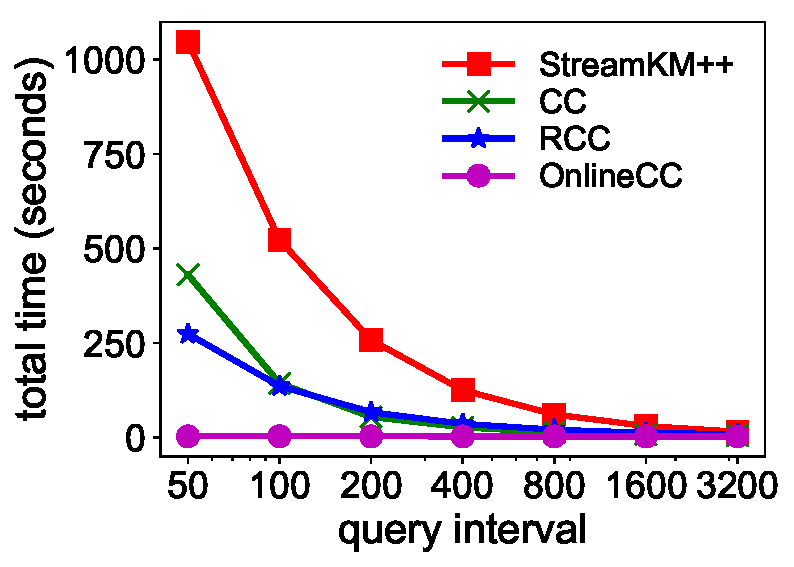
\includegraphics[width=0.23\textwidth]{expfigs/totaltime_q/covtype_total_vs_q.pdf}
  }
  \subfloat[\power]{
  \centering 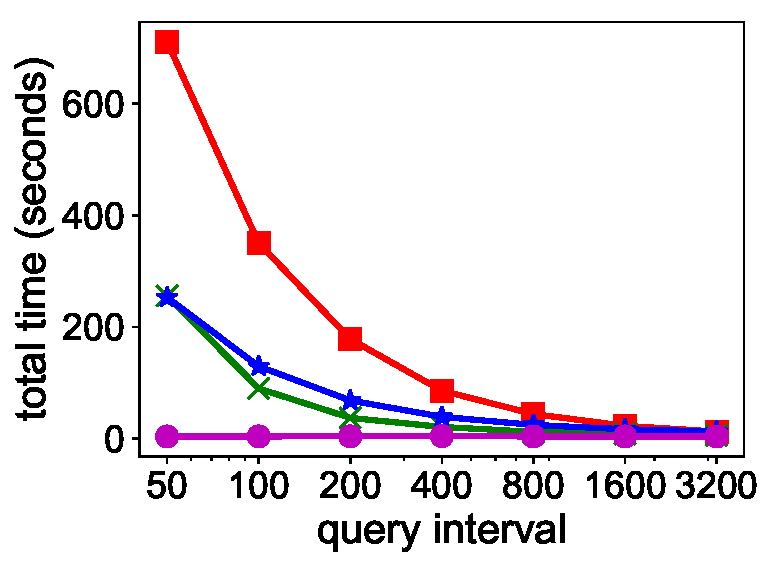
\includegraphics[width=0.23\textwidth]{expfigs/totaltime_q/power_total_vs_q.pdf}
  }
  \subfloat[\intrusion]{
  \centering 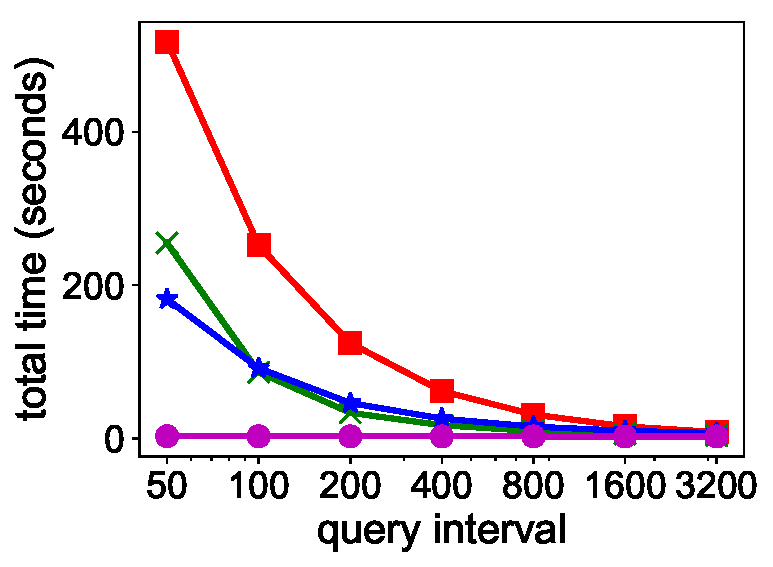
\includegraphics[width=0.23\textwidth]{expfigs/totaltime_q/intrusion_total_vs_q.pdf}
  }
  \subfloat[\drift]{
  \centering 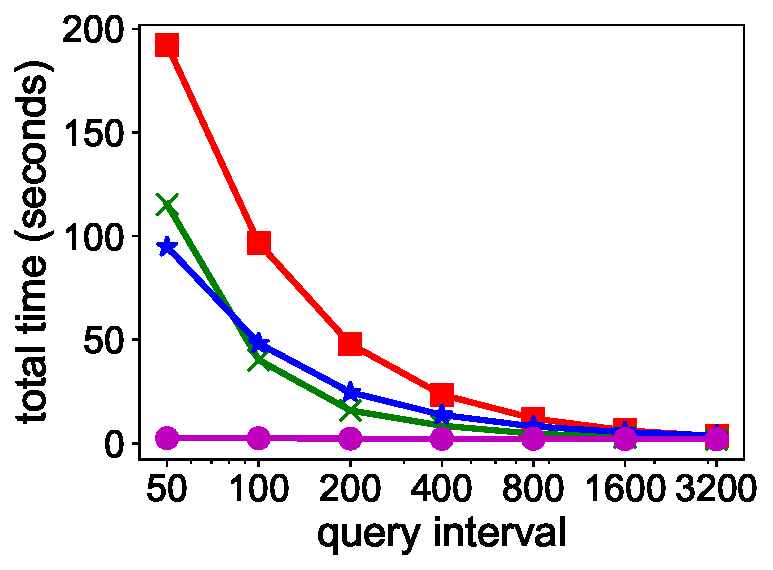
\includegraphics[width=0.23\textwidth]{expfigs/totaltime_q/synthetic_total_vs_q.pdf}
  }
  \caption{Total time (seconds) vs. query interval $q$. The total time is for the entire dataset overall stream. For every $q$ points, there is a query for the cluster centers. The number of centers $k$ is $30$.}
 \label{fig:time-versus-q}
\end{figure*}
%----------------

% metrics vs. bucketsize
%----------------cost vs. bucketsize--------------------
\begin{figure*}
  \centering
  \subfloat[\covtype]{
  \centering 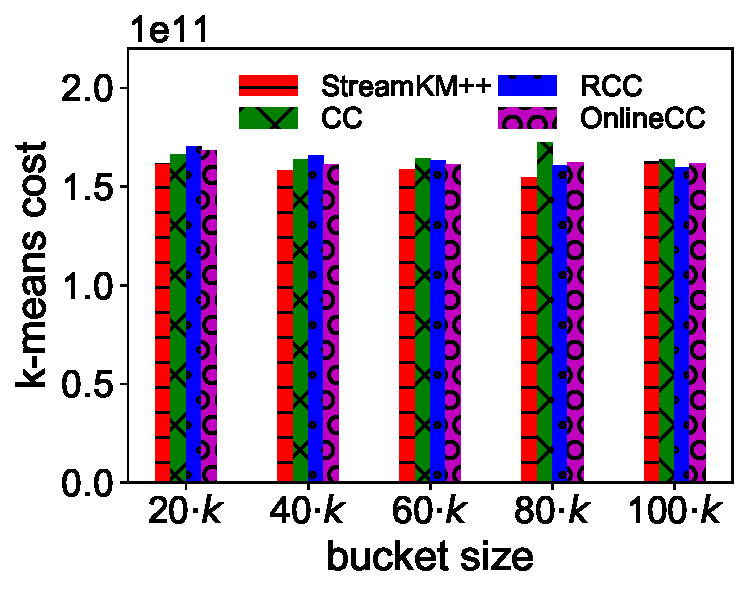
\includegraphics[width=0.23\textwidth]{expfigs/accuracy_bucketsize/covtype_cost_vs_m.pdf}
  }
  \subfloat[\power]{
  \centering 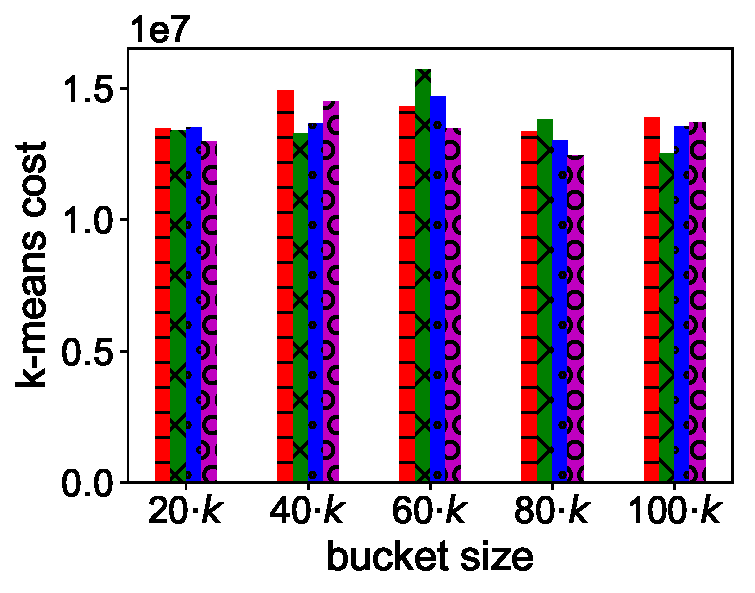
\includegraphics[width=0.23\textwidth]{expfigs/accuracy_bucketsize/power_cost_vs_m.pdf}
  }
  \subfloat[\intrusion]{
  \centering 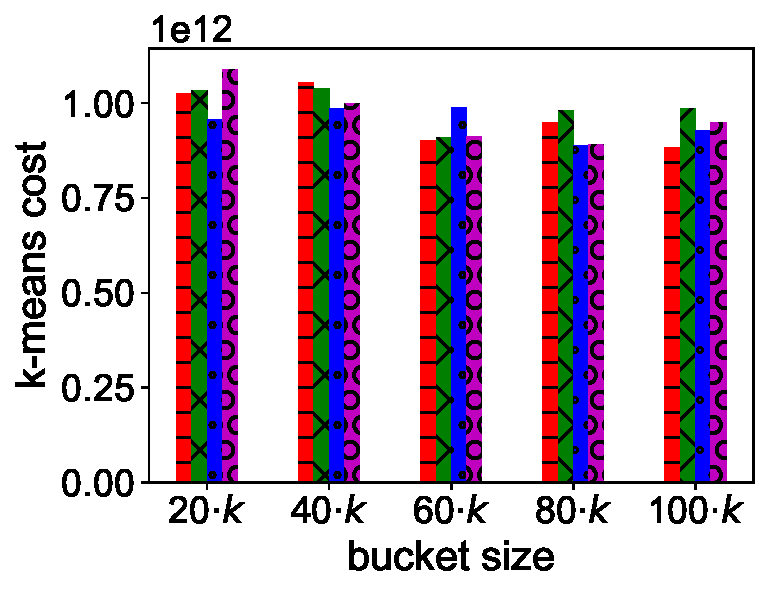
\includegraphics[width=0.23\textwidth]{expfigs/accuracy_bucketsize/intrusion_cost_vs_m.pdf}
  }
  \subfloat[\drift]{
  \centering 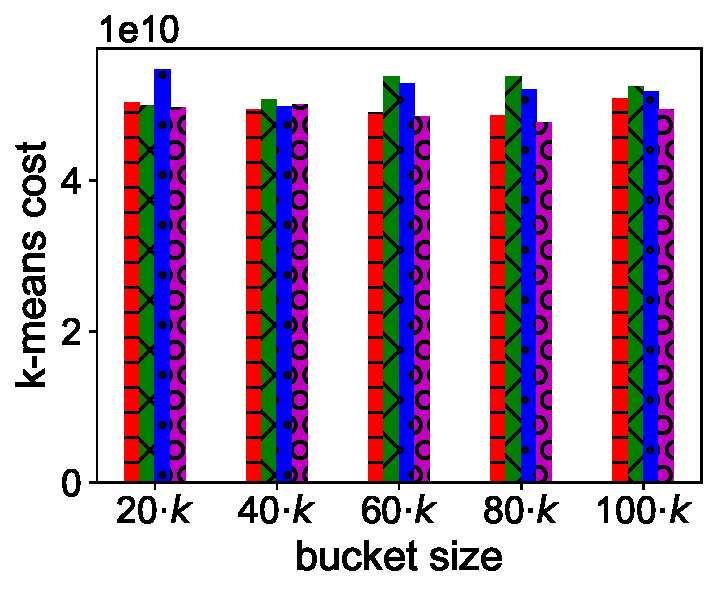
\includegraphics[width=0.23\textwidth]{expfigs/accuracy_bucketsize/synthetic_cost_vs_m.pdf}
  }
  \caption{\km cost vs. bucket size $m$. The cost is computed at the end of observing all the points. The number of clusters $k=30$, query interval $q=100$.  }
 \label{fig:cost-versus-m}
\end{figure*}
%----------------

%----------------update vs. bucketsize--------------------
\begin{figure*}
  \centering
  \subfloat[\covtype]{
  \centering 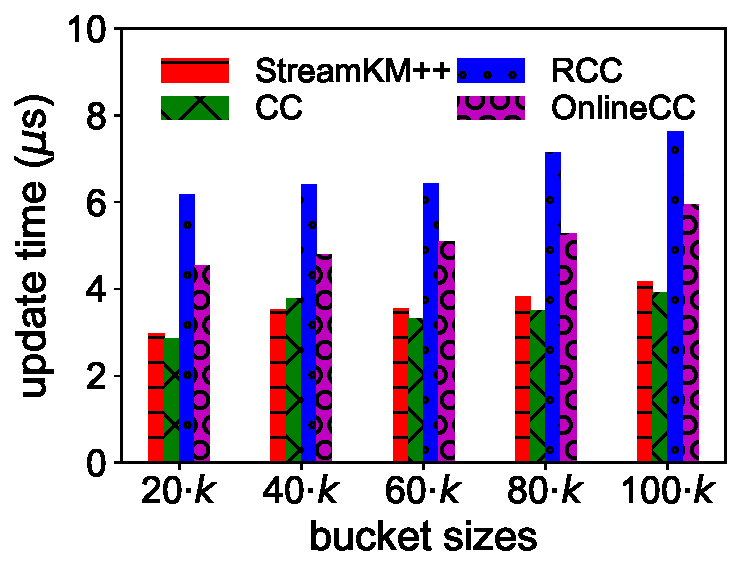
\includegraphics[width=0.23\textwidth]{expfigs/update_bucketsize/covtype_update_vs_m.pdf}
  }
  \subfloat[\power]{
  \centering 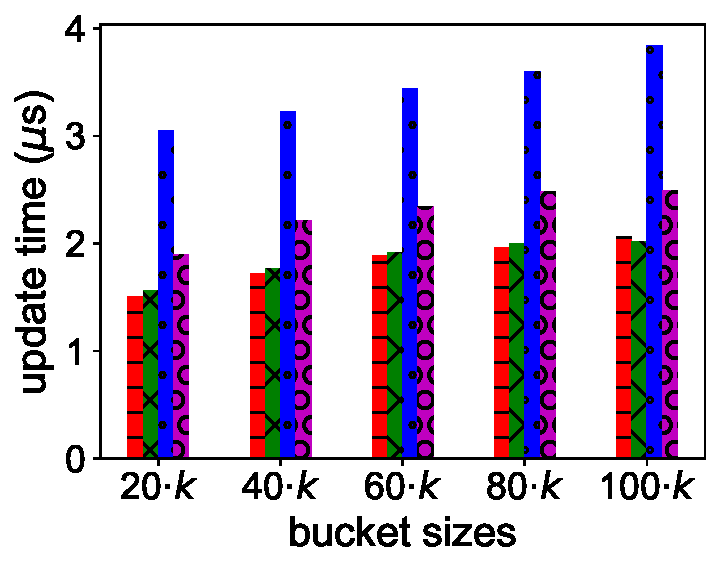
\includegraphics[width=0.23\textwidth]{expfigs/update_bucketsize/power_update_vs_m.pdf}
  }
  \subfloat[\intrusion]{
  \centering 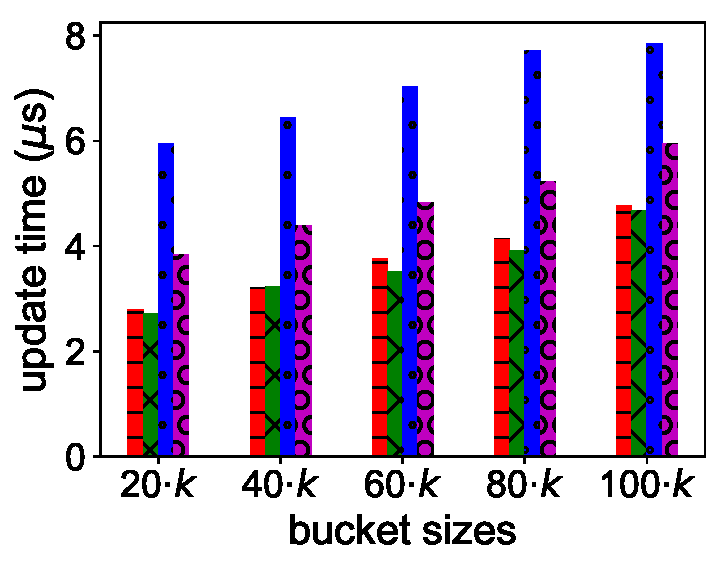
\includegraphics[width=0.23\textwidth]{expfigs/update_bucketsize/intrusion_update_vs_m.pdf}
  }
  \subfloat[\drift]{
  \centering 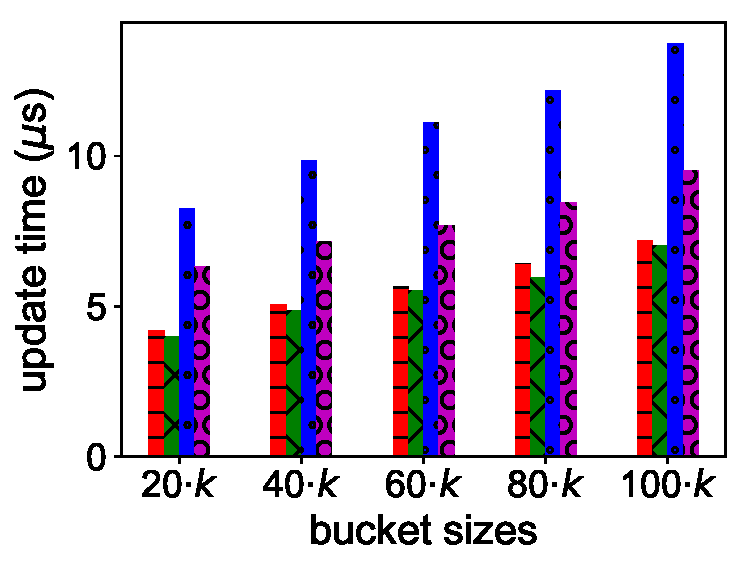
\includegraphics[width=0.23\textwidth]{expfigs/update_bucketsize/synthetic_update_vs_m.pdf}
  }
  \caption{Average update time per point (microseconds)  vs. bucket size $m$. The number of clusters $k=30$, query interval $q=100$.  }
 \label{fig:update-versus-m}
\end{figure*}
%----------------


%----------------query vs. bucketsize--------------------
\begin{figure*}
  \centering
  \subfloat[\covtype]{
  \centering 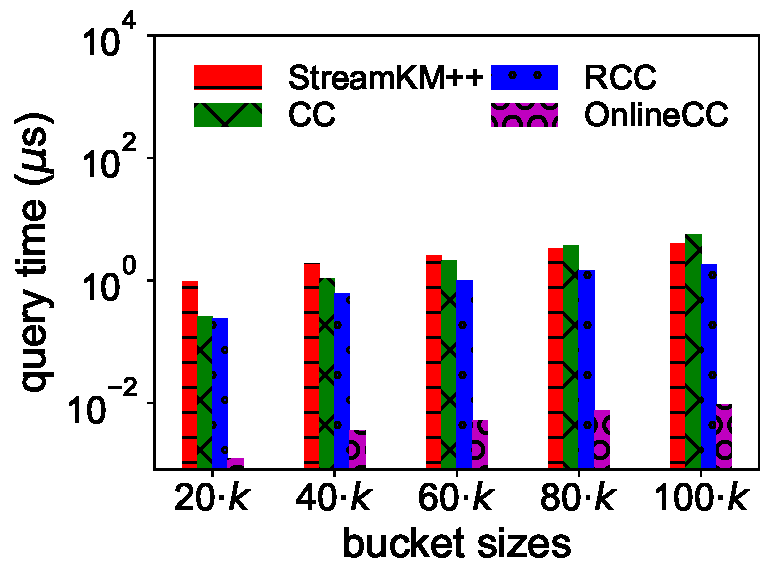
\includegraphics[width=0.23\textwidth]{expfigs/query_bucketsize/covtype_query_vs_m.pdf}
  }
  \subfloat[\power]{
  \centering 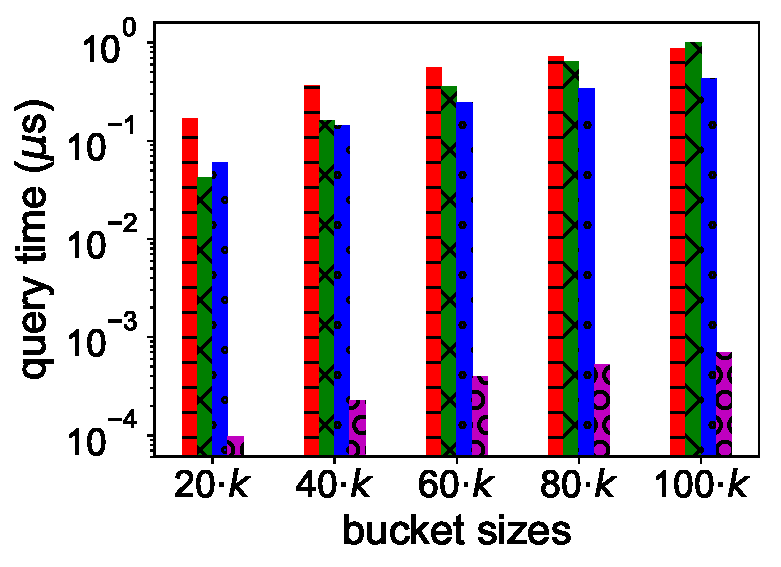
\includegraphics[width=0.23\textwidth]{expfigs/query_bucketsize/power_query_vs_m.pdf}
  }
  \subfloat[\intrusion]{
  \centering 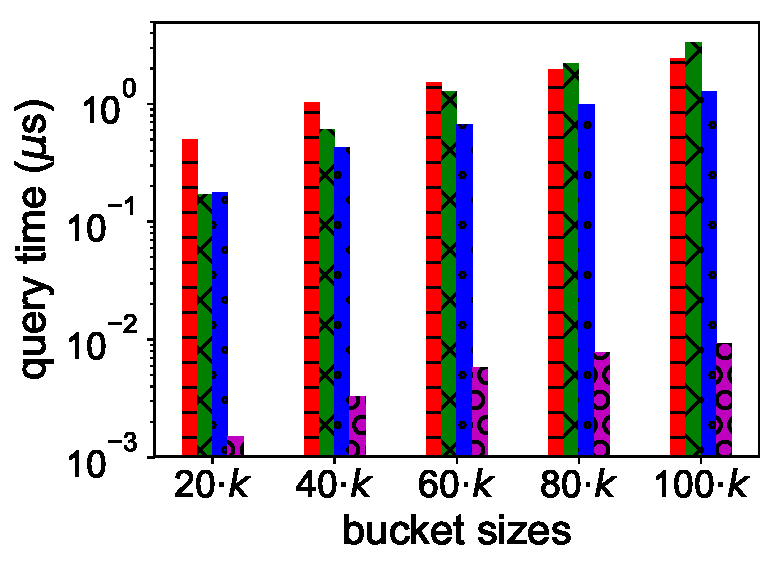
\includegraphics[width=0.23\textwidth]{expfigs/query_bucketsize/intrusion_query_vs_m.pdf}
  }
  \subfloat[\drift]{
  \centering 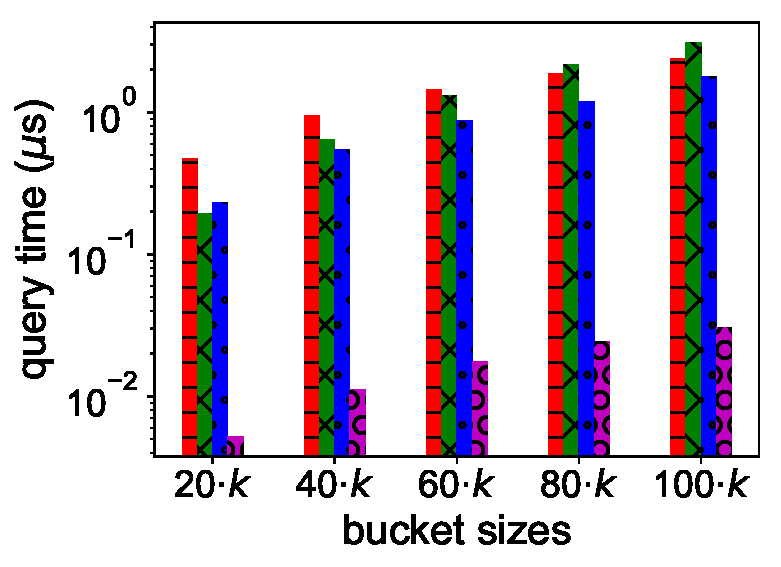
\includegraphics[width=0.23\textwidth]{expfigs/query_bucketsize/synthetic_query_vs_m.pdf}
  }
  \caption{Average query time per point (microseconds) vs. bucket size $m$. The number of clusters $k=30$, query interval $q=100$.  }
 \label{fig:query-versus-m}
\end{figure*}
%-------------------------

%----------------total vs. bucketsize--------------------
\begin{figure*}
  \centering
  \subfloat[\covtype]{
  \centering 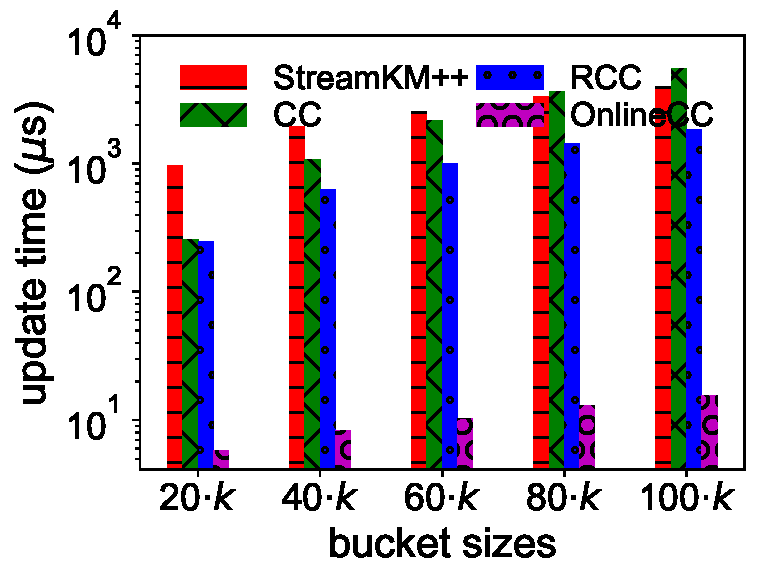
\includegraphics[width=0.23\textwidth]{expfigs/total_bucketsize/covtype_total_vs_m.pdf}
  }
  \subfloat[\power]{
  \centering 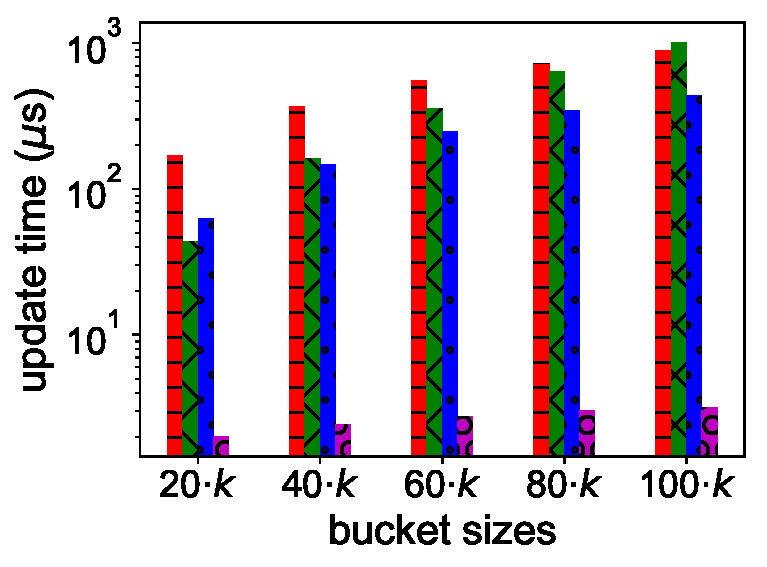
\includegraphics[width=0.23\textwidth]{expfigs/total_bucketsize/power_total_vs_m.pdf}
  }
  \subfloat[\intrusion]{
  \centering 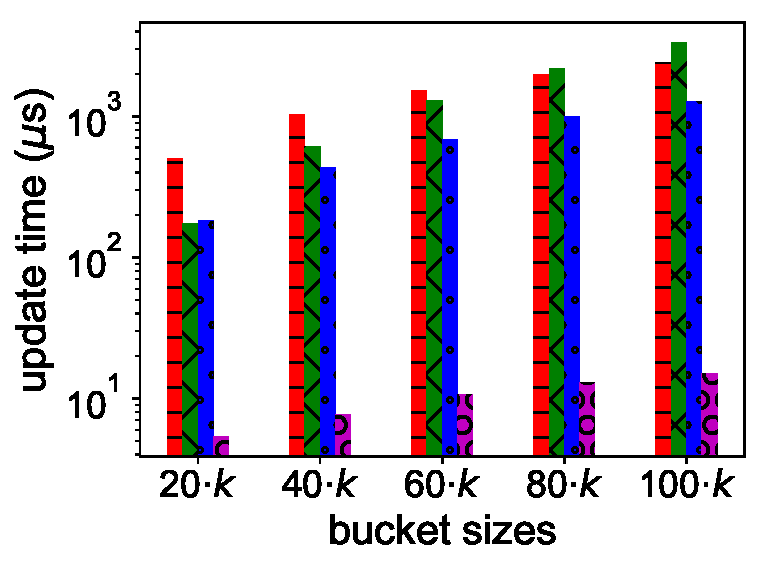
\includegraphics[width=0.23\textwidth]{expfigs/total_bucketsize/intrusion_total_vs_m.pdf}
  }
  \subfloat[\drift]{
  \centering 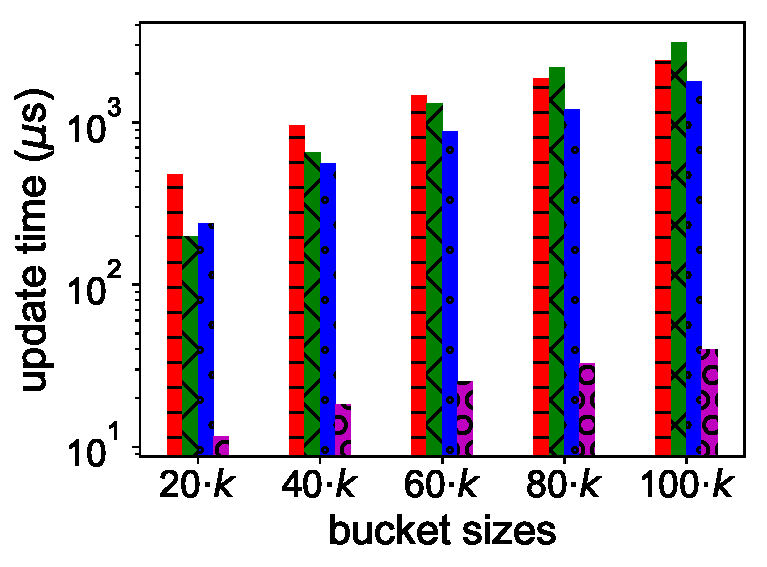
\includegraphics[width=0.23\textwidth]{expfigs/total_bucketsize/synthetic_total_vs_m.pdf}
  }
  \caption{Average runtime per point (microseconds) vs. bucket size $m$. The runtime is the sum of update time (per point) and the query time (per point). The number of clusters $k=30$, query interval $q=100$.  }
 \label{fig:total-versus-m}
\end{figure*}
%-------------------------


% poisson process
%----------------poisson: update time--------------------
\begin{figure*}
  \centering
  \subfloat[\covtype]{
  \centering 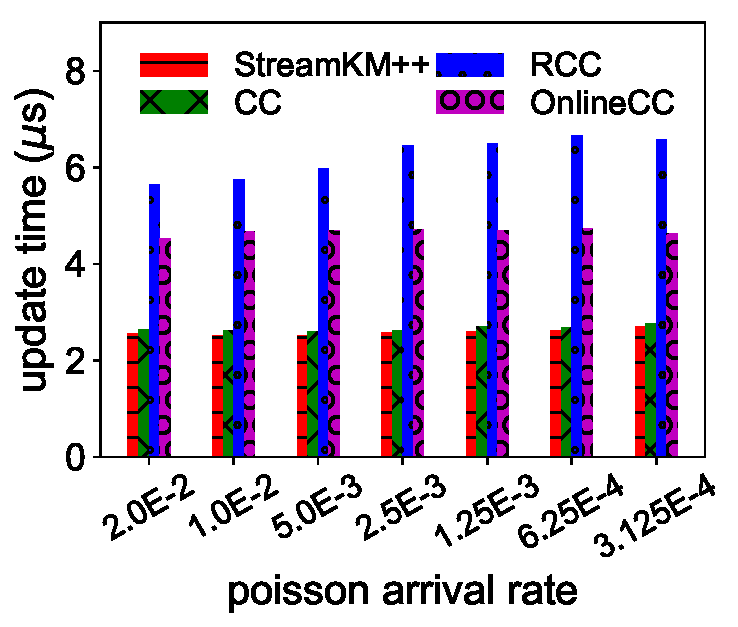
\includegraphics[width=0.23\textwidth]{expfigs/poisson/update/covtype_update_vs_rate.pdf}
  }
  \subfloat[\power]{
  \centering 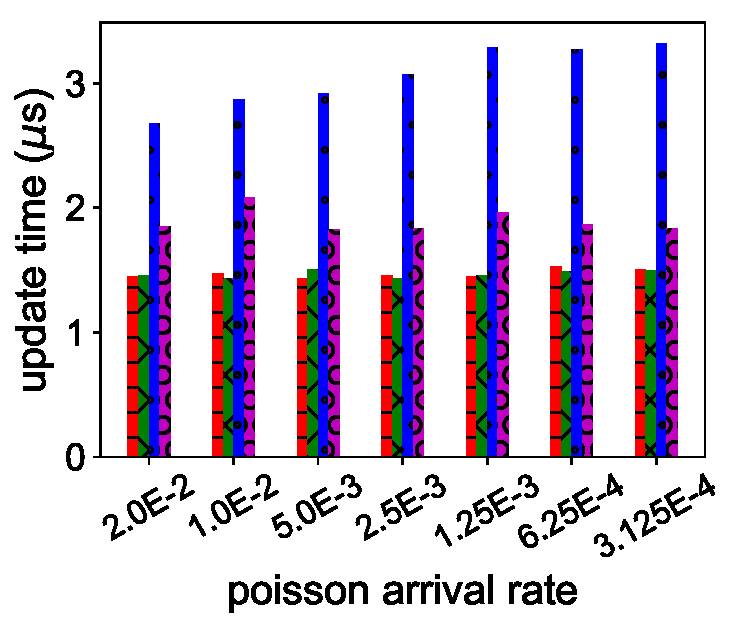
\includegraphics[width=0.23\textwidth]{expfigs/poisson/update/power_update_vs_rate.pdf}
  }
  \subfloat[\intrusion]{
  \centering 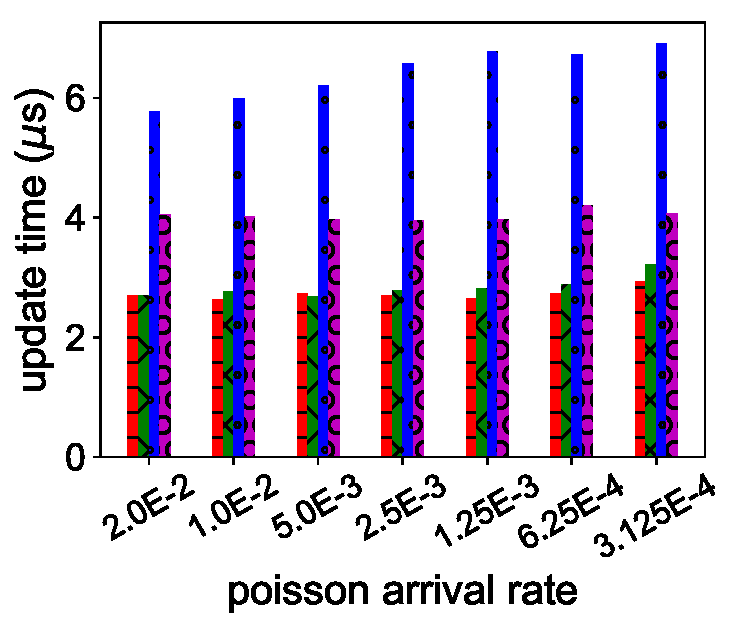
\includegraphics[width=0.23\textwidth]{expfigs/poisson/update/intrusion_update_vs_rate.pdf}
  }
  \subfloat[\drift]{
  \centering 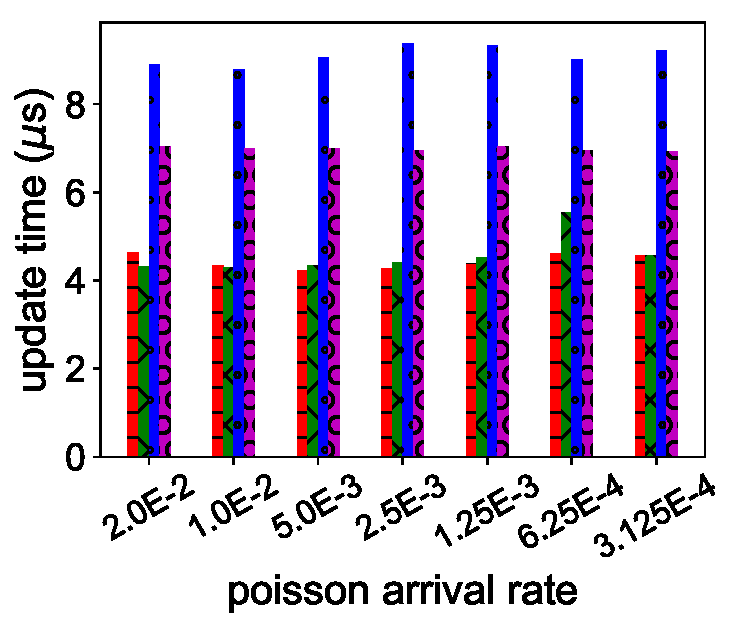
\includegraphics[width=0.23\textwidth]{expfigs/poisson/update/synthetic_update_vs_rate.pdf}
  }
  \caption{Update time per point (microseconds)  vs. poisson arrival rate $\lambda$. }
 \label{fig:poisson-update}
\end{figure*}
%------------------

%----------------poisson: query time--------------------
\begin{figure*}
  \centering
  \subfloat[\covtype]{
  \centering 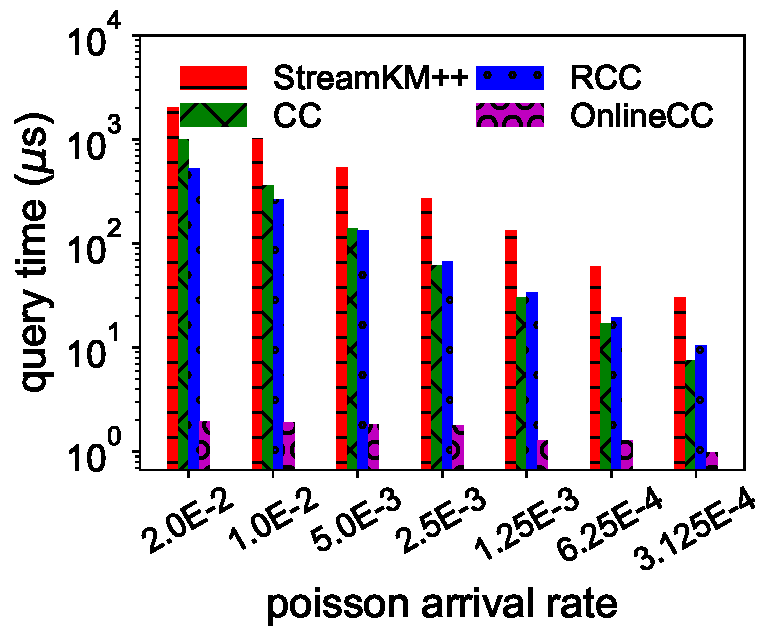
\includegraphics[width=0.23\textwidth]{expfigs/poisson/query/covtype_query_vs_rate.pdf}
  }
  \subfloat[\power]{
  \centering 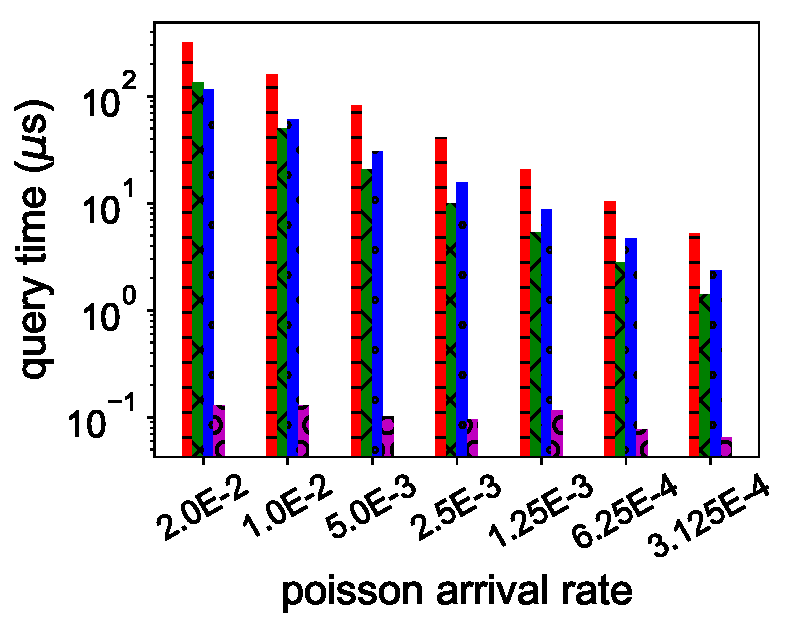
\includegraphics[width=0.23\textwidth]{expfigs/poisson/query/power_query_vs_rate.pdf}
  }
  \subfloat[\intrusion]{
  \centering \includegraphics[width=0.23\textwidth]{expfigs/poisson/query/intrusion_query_vs_rate.pdf}
  }
  \subfloat[\drift]{
  \centering \includegraphics[width=0.23\textwidth]{expfigs/poisson/query/synthetic_query_vs_rate.pdf}
  }
  \caption{Query time per point (microseconds)  vs. poisson arrival rate $\lambda$.}
 \label{fig:poisson-query}
\end{figure*}
%------------------

%----------------poisson: total time--------------------
\begin{figure*}
  \centering
  \subfloat[\covtype]{
  \centering \includegraphics[width=0.23\textwidth]{expfigs/poisson/total/covtype_total_vs_rate.pdf}
  }
  \subfloat[\power]{
  \centering \includegraphics[width=0.23\textwidth]{expfigs/poisson/total/power_total_vs_rate.pdf}
  }
  \subfloat[\intrusion]{
  \centering \includegraphics[width=0.23\textwidth]{expfigs/poisson/total/intrusion_total_vs_rate.pdf}
  }
  \subfloat[\drift]{
  \centering \includegraphics[width=0.23\textwidth]{expfigs/poisson/total/synthetic_total_vs_rate.pdf}
  }
  \caption{Total time per point (microseconds)  vs. poisson arrival rate $\lambda$.}
 \label{fig:poisson-total}
\end{figure*}
%------------------

% onlinecc vs. threshold (switch threshold)
%%----------------cost vs. threshold--------------------
%\begin{figure*}
%  \centering
%  \subfloat[\covtype]{
%  \centering \includegraphics[width=0.23\textwidth]{expfigs/accuracy_bucketsize/covtype_cost_vs_m.pdf}
%  }
%  \subfloat[\power]{
%  \centering \includegraphics[width=0.23\textwidth]{expfigs/accuracy_bucketsize/power_cost_vs_m.pdf}
%  }
%  \subfloat[\intrusion]{
%  \centering \includegraphics[width=0.23\textwidth]{expfigs/accuracy_bucketsize/intrusion_cost_vs_m.pdf}
%  }
%  \subfloat[\drift]{
%  \centering \includegraphics[width=0.23\textwidth]{expfigs/accuracy_bucketsize/synthetic_cost_vs_m.pdf}
%  }
%  \caption{\km cost vs. bucket size $m$. The cost is computed at the end of observing all the points. The number of clusters $k=30$, query interval $q=100$.  }
% \label{fig:cost-versus-m}
%\end{figure*}
%%----------------

%----------------time vs. threshold--------------------
\begin{figure*}
  \centering
  \subfloat[\covtype]{
  \centering \includegraphics[width=0.23\textwidth]{expfigs/onlinecc_time/covtype_time.pdf}
  }
  \subfloat[\power]{
  \centering \includegraphics[width=0.23\textwidth]{expfigs/onlinecc_time/power_time.pdf}
  }
  \subfloat[\intrusion]{
  \centering \includegraphics[width=0.23\textwidth]{expfigs/onlinecc_time/intrusion_time.pdf}
  }
  \subfloat[\drift]{
  \centering \includegraphics[width=0.23\textwidth]{expfigs/onlinecc_time/synthetic_time.pdf}
  }
  \caption{Total runtime (seconds)  vs. switch threshold $\alpha$ in \hybrid algorithm. 
  The number of clusters $k=30$, query interval $q=100$.  
  The update and query time are both counted for the whole stream instead of per point.}
 \label{fig:time-versus-threshold}
\end{figure*}
%----------------

% memory cost
%-------------
\begin{table*}
{ 
\small
\centering
\begin{tabular}
{|c|c c c c| c c c c|}
\hline
\multirow{2}{*}{Dataset} & \multicolumn{4}{ c| }{Memory cost in points}  & \multicolumn{4}{ c| }{Memory cost in Megabytes (MB)} \\  \cline{2-9}
& \skmpp & \cc & \rcc & \hybrid  & \skmpp & \cc & \rcc & \hybrid \\  \hline
\covtype  & 5950  & 11350  & 36550  & 11380  & 2.57 & 4.90  & 15.78  & 4.92  \\   \hline
\power  & 7150  & 13750  & 68950  & 13780  & 0.40  & 0.77  & 3.86  & 0.77  \\   \hline
\intrusion  & 5950  & 11350  & 32950  & 11380  & 1.62 & 3.09  & 8.96  & 3.10  \\   \hline
\drift  & 5350  & 10150  & 20950  & 10180 & 2.91 & 5.52  & 11.40  & 5.54   \\   \hline
\end{tabular}
\smallskip
\caption{Memory cost of algorithms, number of clusters $k$ is set to $30$ .}
\label{table:memory-cost}
}
\end{table*}
%------------



%-----------------------------------------------------
\subsection{Discussion of Experimental Results}
%-----------------------------------------------------
% cost vs. stream
%{\bf Accuracy ($k$-means cost) vs. stream:} 
%We first study algorithms performance versus the stream. 
%Figure~\ref{fig:cost-versus-stream} shows the \km cost of algorithms 
%with more points received from the stream.
%The sequential algorithm has distinct higher (approximately twice) \km cost, compared to other algorithms.  
%This is as expected because the sequential clustering method does not have any guarantee on the clustering quality. 
%However, \skmpp, \cc, and \rcc all yield very similar \km costs on both datasets.  
%This is a different trend from the theoretical results.  According to the theory, 
%with a large merge threshold, the number of levels in the coreset tree decreases, 
%which should lead to better clustering accuracy. With this reasoning, \rcc should achieve 
%the lowest clustering cost as it uses a much larger merge threshold in the coreset tree.  

%{\bf Runtime vs. stream:} 
%Figure~\ref{fig:time-versus-stream} shows the amortized runtime per point versus the stream. 
%We observe that for \skmpp, the average runtime per point increases with the stream. 
%This is because the query cost of \skmpp is related with the depth of the coreset tree, 
%which increases as more points are inserted.
%In contrast, all the other three algorithms keep the runtime per point invariant. 
%This is due to the constant number of coresets merged by using the cache.
%Overall, \hybrid algorithm achieves much faster runtime than others, 
%as it is able to directly retrieve the cluster centers from the online maintained model. 

% cost vs. k
{\bf Accuracy (\km cost) vs. $k$:} Figures~\ref{fig:cost-versus-k} 
shows the result of \km cost under different number of clusters $k$. 
Note that for the \intrusion data, the result of \seqkm is not shown 
since the cost is much larger (by a factor of about ${10}^4$) than 
the other algorithms. Not surprisingly, for all the algorithms studied, 
the clustering cost decreases with $k$. 
For all the datasets, \seqkm always achieves distinct higher \km cost than other algorithms. 
This shows that \seqkm is consistently worse than the other algorithms, 
when it comes to clustering accuracy---this is as expected, since
unlike the other algorithms, \seqkm does not have a theoretical guarantee on
clustering quality.

The other algorithms, \skmpp, \cc, \rcc, and \hybrid all achieve very similar
clustering cost, on all datasets. In Figure~\ref{fig:cost-versus-k}, we also
show the cost of running a batch algorithm \kmpp (followed by Lloyd's iterations). 
We found that the clustering costs of the streaming algorithms are nearly 
the same as that of running the batch algorithm, which can see the input all at once! 
Indeed, we cannot expect the streaming clustering algorithms to perform any better than this.

Theoretically, it was shown that clustering accuracy improves with the merge
degree.  Hence, \rcc should have the best clustering accuracy (lowest
clustering cost). But we do not observe such behaviors experimentally; 
\rcc and \skmpp show similar accuracy. However their accuracy matches that of batch \kmpp. 
A possible reason for this may be that our theoretical analysis of streaming
clustering methods is too conservative. 
\remove{
and/or there is some structure within the 
real data that we can better exploit to predict clustering accuracy.
}

% update vs. k
\noindent{\bf Update Time vs. $k$:} Figure~\ref{fig:update-versus-k} shows the average
update time per point under different number of clusters. 
We first observe that for all the algorithms, the update time increases with the number of centers, 
as from the theoretical result, amortized update time per point is proportional to the bucket size $m$, 
which equals $20 \cdot k$. 
Algorithms \skmpp and \cc have similar update time as both are having exactly the same update process. 
Algorithm \hybrid has higher update time about two times than other algorithms, 
since it runs the update processes of both \seqkm and \skmpp.
Among all the four algorithms compared, \rcc has the highest update time, 
because it updates the \rcc data structure in each order.

% query vs. k
\noindent{\bf Query Time vs. $k$:} Figure~\ref{fig:query-versus-k} shows 
the average query time per point under different number of clusters, 
when the query interval is $100$ points.  Note that the y-axis is in the log scale. 
We see that \hybrid is significantly faster than the rest of algorithms, 
followed by \rcc,  \cc and finally by \skmpp.
\hybrid is about two orders of magnitude faster than \skmpp. 
This shows that the algorithm succeeds in achieving significantly 
faster queries than \skmpp, while maintaining the same clustering accuracy. 
We also note that, when comparing the update time and query time, query time is 
significantly higher than the update time, roughly in three orders of magnitude. 
Thus, it reveals the time reduction on the query time is more important in improving 
the runtime performance. 

% total vs. k
\noindent{\bf Runtime vs. $k$:} Figure~\ref{fig:total-versus-k} shows the average
runtime per point (sum of the update time and query time) under different cluster centers. 
For all the algorithms except \hybrid, we observe that the runtime 
is close to the query time, as the query time dominates the update time. 
For \hybrid, however, the total time is obviously greater than the query time, 
but still much faster (approximately in two orders) than other algorithms.

% metrics vs. q
\noindent{\bf Total Runtime vs. Query Interval:} 
We next consider the effect of different query intervals on the runtime. 
Figure~\ref{fig:time-versus-q} shows the total runtime throughout the 
whole stream as a function of the query interval $q$. 
We note that the total time for \hybrid is consistently the smallest, and does not
change with an increase in $q$. This is because \hybrid essentially maintains
the cluster centers on a continuous basis, while occasionally falling back to
\cc to recompute coresets, to improve its accuracy. For the other algorithms,
including \cc, \rcc, and \skmpp, the query time and the total time decrease as
$q$ increases (and queries become less frequent).
\cc and \rcc have similar total runtime and achieve half of the runtime of \skmpp, 
by using the cache. 
All the algorithms converge their total runtime when the queries are very less frequent,
that $q$ is more than $1600$ points.

% metrics vs. bucketsize
\noindent\textbf{Metrics vs. Bucket Size:} 
We measure the performance of algorithms under different bucket sizes. 
The bucket size ranges from $20 \cdot k$ to $100 \cdot k$, where $k$ is 
the number of clusters and set to $30$.
Figure~\ref{fig:cost-versus-m} compares the \km cost of different algorithms.
The accuracy is similar with different bucket sizes, even though in theory, it should 
have better accuracy with larger bucket sizes. This observation matches the results 
in \cite{AMR+12}, that for most cases in practice, bucket size of $20 \cdot k$ is a good number 
for \skmpp on clustering accuracy. For our algorithms with coreset caching, the same
parameter setting on bucket size applies.
Figure~\ref{fig:update-versus-m}, ~\ref{fig:query-versus-m} and ~\ref{fig:total-versus-m} 
show the average update time, query time and total time per point respectively.
Our first observation is that all the timing results are increasing with the bucket size, 
as both the update time and query time are proportional to the bucket size.
The second observation is when the bucket size increases over $80 \cdot k$, 
the query time of \cc exceeds the query time of \skmpp. The reason is when 
bucket size increases, the number of buckets received in total becomes smaller 
and in turn the depth of the coreset tree becomes shorter. Thus for \skmpp, 
the number of buckets to merge during the query is trivially different than using 
the cache. Comparing to \skmpp, as \cc uses additional time on inserting new 
coreset to the cache (line $17$ in Algorithm~\ref{algo:cctree-coreset}),
the query time of \cc exceeds \skmpp when bucket size is large. 

% poisson process
\noindent\textbf{Queries in Poisson Process:}
We consider the queries arrive in a poisson process instead of the query interval is in the 
fixed number of points. The average update time per point, query time per point and total 
are shown in Figure~\ref{fig:poisson-update},~\ref{fig:poisson-query} 
and~\ref{fig:poisson-total} respectively, with different value of arrival rate. 
Note that the higher value of arrival rate, means the less frequent queries. 
The update time does not have a changing trend with the increasing value of arrival rate, 
as changing query arrival rate only affects the query process. For all the algorithms,
the query time per point drops down with lower arrival rate, as the less frequent queries. 
Comparing different algorithms, \skmpp uses most query time without caching. 
Under high arrival rate $0.02$ such that the average query interval is $50$ points, 
the query time of \rcc is less than \cc. When the arrival rate decreases, \cc has lower 
query time.  The reason is as follows: generally \rcc needs to merge multiple levels of 
coresets comparing to \cc, which only needs to merge one coreset from coreset tree and 
the other coreset in the cache. However, as \rcc applies multiple levels of caches, the chance that 
successfully finding the target coreset in the cache is much higher than \cc. Thus, when queries 
becomes very frequent, with the help of multiple level of caching, the query time of \rcc is faster than \cc.  
Like what we observed in previous experiments, \hybrid achieves the furthest time in query 
due to the nature of online cluster centers maintenance.
As the query time dominates than the update time, the total runtime per point shown in 
Figure~\ref{fig:poisson-total}, which is summation of the two, has similar trend as query time per point.

% onlinecc metrics vs. threshold
\noindent\textbf{Switching Threshold of \hybrid:}
We consider the impact of switching threshold parameter to the \hybrid algorithm.
The runtime throughout the whole stream is shown in Figure~\ref{fig:time-versus-threshold}. 
From the plot we first observe that runtime decreases with higher value of switching threshold, 
which indicates the looser requirement on the clustering accuracy. We also notice that the runtime 
drops dramatically when changing from $1.2$ to $2.4$, approximately $3$ to $5$ times. 
But much less decrease when the threshold increases further. Thus, the ideal switching threshold value 
for \hybrid algorithm is $2$ to $4$ if it has already fulfilled the requirement on accuracy.

% memory space
\noindent\textbf{Memory Usage:} Finally, we report the memory cost in
Table~\ref{table:memory-cost} using $k=30$; the trends are identical for other
values of $k$. Evidently, \skmpp uses the least memory since it only maintains
the coreset tree. Because it also maintains a coreset cache, \cc requires
additional memory. Even then, \cc's memory cost is less than 2x that of
\skmpp. The memory cost of \hybrid is similar to \cc while \rcc has the highest
memory cost.  This shows that the marked improvements in speed requires only a
modest increase in the memory requirement, making the proposed algorithms
practical and appealing.
